\documentclass[a4paper,12pt]{article}
\usepackage[T1]{fontenc}
\usepackage[czech, english, spanish]{babel}
\usepackage[margin=2.5cm]{geometry}
\usepackage{hyperref}
\usepackage{array}
\usepackage{graphicx}
\usepackage{setspace}
\usepackage{natbib}
\usepackage[toc]{appendix}
\usepackage[export]{adjustbox}
\usepackage{float}
\usepackage{amsmath}
\usepackage{xcolor}
\usepackage{transparent}
\usepackage{listings}

\bibliographystyle{unsrtnat}
\setcitestyle{authoryear,open={(},close={)}}
\AtBeginDocument{\renewcommand{\harvardand}{,}}


\newcommand\tema{Pulzní Oxymetrie}
\newcommand\obor{Informatika}
\newcommand\hlavicka{\noindent
\includegraphics[width=0.993\textwidth]{Formality/Hlavicka.png}\\\\}
\newcommand*{\doi}[1]{\href{https://doi.org/#1}{doi: #1}} 
\hbadness=10000



\begin{document}
%Titulní Strana
\author{Martin~Truksa \and Vojtěch~Tvrdík}
\title{\tema}
\date{2021/2022}
\maketitle

\thispagestyle{empty} 
\newpage

\null
\hlavicka
\begin{tabular}{|>{ \itshape\large}m{0.965\textwidth}|}
\hline
\vspace{0.75cm}
\centerline{\uppercase\expandafter{\tema}}\\
\hline
\end{tabular}
\\\\\\\\\\

\noindent{\large \textbf{Obor:} {\obor\\}
\textbf{Autoři:} {Martin Truksa a Vojtěch Tvrdík}}\\
\\\\\\
\textbf{Třída:} Septima\\
\textbf{Školní rok:} 2021/2022\\
\textbf{Vedoucí práce:} Ing. Jaroslav Šebestík, Ph.D.\\
\textbf{Oponent:} Mgr. Věra Jurčáková\\
\textbf{Rozsah práce (s.):}\par
celkový (včetně této strany, vyjma titulní): 39\par
vlastní text: 26\par
přílohy: 4 + samostatné přiložené soubory (modely, zdrojový kód)\par
vědecký aparát (poznámky, bibliografie aj.): 3\\\\\\\\
\textbf{Formát elektronické podoby práce:} \LaTeX (.tex, .bib, .png, .jpg, .pdf, .pdf\_tex), .pdf\\
\textbf{Formát příloh práce:} .ino, .py, .xlsx, .stl, .blend, .txt

\thispagestyle{empty} 
\newpage

\null
\hlavicka
\setlength\extrarowheight{3pt}
\begin{tabular}{|p{5cm}|p{10cm}|}
\hline
ANOTACE & Tato práce se zabývá pulzní oxymetrií a je rozdělena na tři části. V první části práce byly popsány principy pulzní oxymetrie, její technická implementace a její různá využití. Druhá část se zabývá samotným vývojem oxymetru pro domácí použití. Ve třetí části byla demonstrována funkčnost oxymetru provedením výzkumu obsahu kyslíku v krvi během fyzické aktivity.\\
\hline
KLÍČOVÁ SLOVA & pulzní oxymetrie, \(SpO_2\), hemoglobin, saturace, oxymetr, 3D tisk\\
\hline
\selectlanguage{english}
ANNOTATION & This thesis deals with pulse oximetry and is divided into three parts. In the first part the principles of pulse oximetry, its technical implementation, and its various uses were described. The second part deals with the development of an oximeter for home use. In the third part the functionality of the oximeter was demonstrated by investigating levels of blood oxygen during physical activity.\\
\hline
KEYWORDS & pulse oximetry, \(SpO_2\), hemoglobin, saturation, oximeter, 3D printing\\
\hline
\selectlanguage{spanish}
ANOTACIÓN & Esta tesis trata de la pulsioximetría y se divide en tres partes. En la primera parte, fueron descritos los principios de la pulsioximetría, su aplicación técnica y sus diversos usos. La segunda parte trata del desarrollo de un oxímetro para uso doméstico. En la tercera parte, fue demonstrada la funcionalidad del oxímetro investigando los niveles de oxígeno en la sangre durante una actividad física.\\
\hline
PALABRAS CLAVE & pulsioximetría, \(SpO_2\), hemoglobina, saturación, oxímetro, impresión 3D\\
\hline
\end{tabular}

\selectlanguage{czech}
\thispagestyle{empty} 
\newpage
\setstretch{1.5}

\null \vfill
\section*{Prohlášení}
Prohlašujeme, že jsme svou práci vypracovali samostatně a použili jsme pouze podklady (literaturu, SW atd.) uvedené v přiloženém seznamu. Nemáme závažný důvod proti zpřístupňování této práce v souladu se zákonem č. 121/2000 Sb., o právu autorském, o právech souvisejících s právem autorským a o změně některých zákonů (autorský zákon) v platném znění.\\\\\\

\noindent
V~Praze~dne~24.~března~2022 
\begin{flushright}
........................................\\
\emph{Martin Truksa~~~~~~~~}
\end{flushright}
~\\~\\~
\noindent
V~Praze~dne~24.~března~2022 
\begin{flushright}
........................................\\
\emph{Vojtěch Tvrdík~~~~~~~~}
\end{flushright}

\thispagestyle{empty} 
\newpage

\null
\vfill %odsadí dolů
\section*{Poděkování}
Chtěli bychom poděkovat panu Ing. Jaroslavu Šebestíkovi, Ph.D. za jeho trpělivost a četné konzultace, bez kterých by tato práce nemohla vzniknout, paní Mgr. Věře Jurčákové za její připomínky k práci a cvičební materiály, které poskytla jako podklad pro náš výzkum a Benjaminu Swartovi za jeho asistenci při procesu designování 3D modelů. Velké poděkování patří také vedení naší školy, za peníze na nákup potřebné elektroniky a zprostředkování příležitosti zpracovávat toto téma. V neposlední řadě patří poděkování všem účastníkům našeho výzkumu za jejich účast ve výzkumu a jejich zpětnou vazbu k našemu oxymetru.
\section*{Etické zásady}
Výzkum, který je součástí této práce byl proveden v souladu s etickými zásadami, s nimiž byli jeho účastníci seznámeni. Mezi tyto zásady patří anonymita, dobrovolnost účasti a její odvolatelnost. Účastníci byli též poučeni o ochraně osobních údajů.
\thispagestyle{empty} 
\newpage

%potvrzeni etiky

\thispagestyle{empty} 
\tableofcontents
\thispagestyle{empty} 


\newpage
\part{Úvod}
Pulzní oxymetrie se dostává do života kolem nás, aniž bychom o tom věděli. Ve skutečnosti většina lidí ani přibližně neví, co by si pod tímto slovním spojením měla představit. Přesto je to právě pulzní oxymetrie, která dnes a denně pomáhá lékařům po celém světě s monitorováním pacientů a zachraňováním jejich životů. Nikdy nebyla potřeba zjišťovat rychle a přesně kyslík v krvi tak důležitá, jako právě v současné době.
\par Kvůli pandemii Covidu-19, nemoci způsobené virem SARS-CoV-2, se stalo, že se ve vlnách přeplňovaly nemocnice po celém světě a na jednotkách intenzivní péče docházela místa. Vzhledem k tomu, že SARS-CoV-2, jak už část názvu napovídá (SARS = Severe Acute Respiratory Syndrome), způsobuje potíže s dýcháním, je u pacientů, převážně ve vážnějším stavu, naprosto nezbytné monitorovat saturaci kyslíku v krvi.
\par Kromě tohoto medicínského využití, kde je potřeba velice vysoká přesnost, jsou však ještě další, kde na přesnosti přístroje nezávisí životy pacientů. Běžní uživatelé, ačkoliv potřebují přesné měření, nevyžadují přesnost na úrovni zdravotnických přístrojů a ani jednorázová chyba přístroje je nemůže ohrozit - ať už využívají oxymetr při cvičení pro hlídání zátěže, nebo například zjišťují, jestli nemají ve spánku problém s dýcháním. Pro tyto účely se na trhu v současnosti vyskytují dva typy produktů.
\par Prvním z nich jsou chytré hodinky a náramky: když si člověk vybaví chytré hodinky, je velká šance, že si je představí se svítícím zeleným světýlkem v části, která přiléhá na ruku. To je právě jedna z diod, která má za úkol zjišťovat pulz a saturaci kyslíku v krvi. Nevýhodou těchto produktů je však jejich cena, spojená se všemi funkcemi, které s sebou chytré hodinky nesou. Nejsou tedy například vhodné, pokud se člověk rozhodne je využít pro sledování spánku svého staršího příbuzného.
\par Druhým typem produktu jsou samostatné pulzní oxymetry, které jsou, zjednodušeně řečeno, tak přesné, jak jen může běžný uživatel potřebovat. I jejich cena je relativně přijatelná - v současnosti se pohybuje v řádu vyšších stovek korun. I tyto oxymetry jsou však pro většinu uživatelů přesnější, než kdy využijí, což znamená, že se cena dá ještě snížit použitím domácky vyrobeného oxymetru.
\par V teoretické části této práce detailně vysvětlíme, jak pulzní oxymetrie funguje, jakých principů využívá a jak se zpracovávají naměřená data, a rozebereme její využití v reálném životě - od profesionálního vybavení, až po nejobyčejnější nepravidelné kontrolování pulzu. V praktické části následně provedeme čtenáře postupem při vyvíjení „domácího“ oxymetru, od volby platformy, přes 3D tisk, až po software. Návod na stavbu je včetně všech tipů zveřejněn pod open-sourcovou licencí na webu, aby kdokoliv mohl s běžně dostupnými součástmi a za velice dobrou cenu postavit svůj vlastní oxymetr a následně si ho upravit pro své specifické potřeby.
\par Tento pulzní oxymetr bude také v rámci práce vyzkoušen v rámci výzkumu týkajícího se obsahu kyslíku v krvi v závislosti na fyzické námaze. Cílem výzkumu nebude přinést nové poznatky a nová data, ale demonstrovat funkčnost výsledného produktu a způsob zacházení s ním.


\newpage
\part{Teoretická Část}

\section {Pulzní oxymetrie}
\subsection {Historie}
Pulzní oxymetrie je neinvazivní optická technika měření saturace kyslíku v cévách ($SpO_2$). Historie této metody sahá do dob před druhou světovou válkou. Německý lékař a univerzitní profesor Karl Matthes se již od roku 1929, kdy získal doktorát svou prací o zpomalování pulzu morfiem, zabýval oběhovou soustavou. Roku 1935 představil svoji metodu, „\emph{jež umožňuje průběžné zaznamenávání arteriální saturace kyslíkem v lidech způsobem nevyžadujícím krev}". Tuto metodu využíval pro měření plicní kapacity a jako ukazatel metabolického stavu člověka, což však byly v té době již vyřešené problémy. \citep{matthes}
\par Prací na pulzní oxymetrii se však nejvíce proslavil americký fyziolog Glenn Allen Millikan, který vyvinul přístroj fungující na principech Matthesova přístroje, který se připevňoval na ušní lalůček. Pomocí světla průběžně měřil přibližnou saturaci krve kyslíkem u armádních pilotů při letech ve velkých výškách. \citep{TremperPulseOximetry}
\par Tento přístroj, který sloužil jako senzor pro kyslíkovou masku sestával z „\emph{miniaturní žárovky, dvou barevných filtrů a dvou fotočlánků se selenovým přechodem, vážil 30 gramů a nasazoval se přes ucho. Jeden z těchto filtrů propouštěl světlo o vlnové délce, která je stejně pohlcována oxy- a deoxy- hemoglobinem, což zajišťovalo měření celkového množství hemoglobinu v cestě od zdroje světla nehledě na jeho saturaci kyslíkem. Druhá barva byla absorbována těmito dvěma druhy hemoglobinu ve velmi rozdílném množství,}“ díky čemuž se dala dopočítat celková saturace kyslíku v krvi pilota tak, aby kyslíková maska v případě potřeby dodávala správné množství kyslíku. \citep{1942oximeter}
\par Tato převratná metoda se však rozšířila až v 80. letech minulého století, kdy na sálech a jednotkách intenzivní péče doplnila tehdy používanou analýzu parciálního tlaku kyslíku ($PO_2$). Tato metoda se využívala v kombinaci s fyzickými ukazateli, jako například zbarvení kůže do modra, které však kvůli své subjektivitě nebyly vhodné. Ani samo měření $PO_2$ však nebylo optimální metodou - vztah mezi $PO_2$ a saturací kyslíkem totiž není lineární, což znamená, že nebylo snadné výsledky snadno, rychle a správně interpretovat. Kombinace oxymetrie s měřením parciálního tlaku kyslíku přetrvala do současnosti, kdy se pacientovi v anestezii nebo na jednotce intenzivní péče měří saturace průběžnou pulzní oxymetrií v kombinaci s přerušovaným měřením $PO_2$ pomocí analyzátorů krevních plynů. \citep{KYRIACOU}
\begin{figure}[H]
  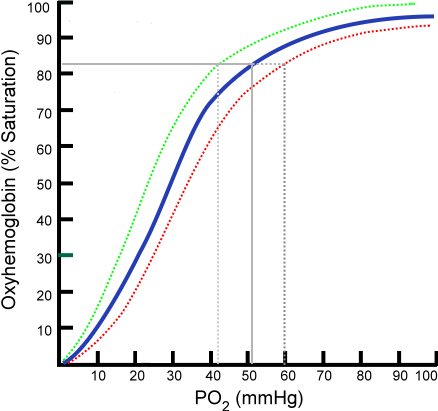
\includegraphics[scale=1, center]{Kapitoly/Teoreticka/Obrazky/TlakKysliku.png}
  \caption [Vztah mezi $PO_2$ a saturací kyslíku v krvi]{Vztah mezi $PO_2$ a saturací kyslíku v krvi, který byl před vynalezením metody pulzní oxymetrie využívaný, není lineární a tudíž nebylo snadné rychle a správně naměřené hodnoty interpretovat. \citep{ratznium_2006}, upraveno}
  \label{fig:PO2}
\end{figure}
\par Pulzní oxymetrie však v současnosti není již specializovanou metodou pro vojenské či zdravotnické účely, ale je používána i v zařízeních určených běžným uživatelům, a to nejen samostatně, ale i jakožto součást komplexnějších produktů. Oproti původnímu Millikanovu oxymetru navíc používáme přesnějších zdrojů světla, LED světlech o specifických vlnových délkách. Zároveň se dá měřit i na jiných částech těla, než je ucho - běžně dostupné oxymetry nejčastěji měří na prstu, existují však i varianty měřící na zápěstí.
\subsection {Princip fungování}
Srdce člověka, jak je obecně známo, funguje v cyklech. Pro krev v tepnách to znamená, že ve chvíli, kdy srdce vypuzuje krev, se zvýší její objem díky elasticitě tepen. Zvýšení tohoto objemu logicky vede k nižší propustnosti světla, díky čemuž mají pulzní oxymetry schopnost měřit srdeční tep.
\par Saturace kyslíku je pak udávána vztahem $SpO_2 = \frac{HbO_2}{\text{Hemoglobin celkem}}$, kde $HbO_2$ je oxyhemoglobin. Tento vztah se pro běžné měření oxymetrem, který umí rozlišovat jen mezi dvěma základními formami hemoglobinu, zjednodušuje na $SpO_2 = \frac{HbO_2}{HbO_2+Hb}$, kde $Hb$ je deoxyhemoglobin). Nové pokročilejší přístroje jsou však schopny detekovat i další formy hemoglobinu - karboxyhemoglobin a methemoglobin. Rovnice pro takovéto měření je pak $SpO_2 = \frac{HbO_2}{HbO_2+Hb+HbCO+HbMet}$, kde $HbCO$ je karboxyhemoglobin a $HbMet$ je methemoglobin. 
\subsubsection{Aplikace Lambertova-Beerova zákona} Samotné měření saturace kyslíku v krvi pak probíhá na principu Lambertova-Beerova zákona, který popisuje pohlcováni elektromagnetické záření. Aplikace tohoto zákona je popsána v následujících rovnicích, které popisuje \cite{KYRIACOU}.
\begin{equation}%když budeš chtít víc rovnic u sebe alignnout, tak je to align místo equation a před alignnutý = dáš &
  {\epsilon_{\lambda}cl} = A_{\lambda} = ln(\frac{I_s}{I_d})  
\end{equation}\\
Text1\\
\begin{equation}
    A_{\lambda} = ln(\frac{I_d+AC_{\lambda}}{I_d})
    \label{EQ:ZAKLAD}
\end{equation}\\
Text2, příklad reference na rovnici \ref{EQ:ZAKLAD}.\\
\begin{equation}
    A_{\lambda} = ln(1+\frac{AC_{\lambda}}{I_d}) \simeq \frac{AC_{\lambda}}{I_d}
\end{equation}\\
Text3\\
\begin{equation}
    \frac{AC_{\lambda}}{I_d} = A_{\lambda} = \frac{AC_{\lambda}}{DC_{\lambda}}
\end{equation}\\
Text4\\

\subsubsection{Volba vlnových délek}
 
%\begin{figure}[H]
%  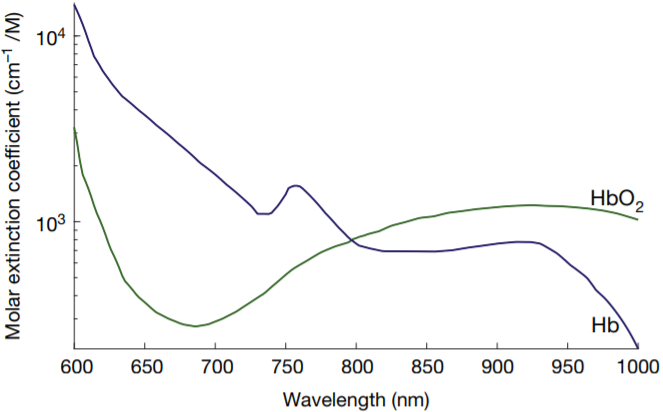
\includegraphics[scale=1, center]{Kapitoly/Teoreticka/Obrazky/Absorpce.png}
%  \caption [Absorpční spektrum HHb a Hb$O_2$]{Absorpční spektrum HHb a Hb$O_2$, na přibližně 805 nanometrech je absorpce stejná, na nižších vlnových délkách absorpci způsobuje převážně HHb, na vyšších pak Hb$O_2$. \citep{KYRIACOU}, upraveno}
%  \label{fig:Absorpce}
%\end{figure}

\subsection {Běžně využívané metody}
Při využívání pulzní oxymetrie jsou 2 různá uspořádání elektroniky využívané pro měření. Jedná se o transmisní a reflektanční měření, která jsou schematicky znázorněna v obrázku \ref{fig:Metody}. Každý z těchto typů měření, jak už jejich názvy napovídají, využívá jiné trajektorie světla skrze prst, což přináší své výhody i nevýhody.
%\begin{figure}[H]
%  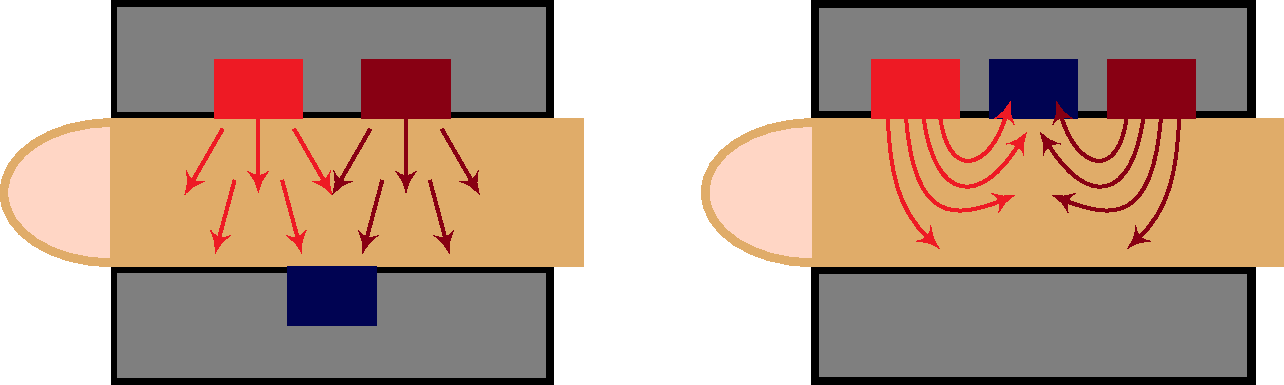
\includegraphics[scale=1, center]{Kapitoly/Teoreticka/Obrazky/Metody.svg}
%  \caption []{}
%  \label{fig:Metody}
%\end{figure}
\par \textbf{Transmisní metoda} měření spočívá v měření světla, které projde skrz tkáň, což v praxi znamená, že se na kůži z jedné strany svítí oběma diodami a fotodioda se nachází naproti nim. Hlavní výhodou tohoto způsobu měření je vysoká přesnost výsledného měření, které je dosaženo převážně díky přímé trajektorii světla, kdy nezáleží na jeho odrazu od prstu. Naopak hlavní nevýhodou této metody je relativně omezené množství materiálu mezi diodami a fotodiodou, protože při větším množství tkáně v trase světla by již nedocházelo k dostatečnému přenosu světla pro přesné určení saturace. Tato metoda se tedy využívá při měření přes prst, případně ušní lalůček. % Nakreslit obrázek
\par \textbf{Reflektanční metoda} měření naopak využívá světla odraženého tkáněmi pod kůží. To v praxi znamená, že se všechny 3 komponenty (obě LED a fotodioda) nachází na jedné straně ruky (případně jiné části těla), a to tak, že fotodioda se nachází mezi oběma LED, aby se vlivem nerovné vzdálenosti nezkreslovala intenzita záření. Výhodou tohoto měření je, že oxymetr využívající tohoto principu je výrazně přenosnější a pohodlnější pro uživatele, vzhledem k tomu, že ho stačí pouze přiložit. Z tohoto důvodu se využívá ve fitness náramcích a hodinkách, kde by nebylo praktické mít dvě pevné části naproti sobě. Nevýhodou je však nižší přesnost měření, která je převážně důsledkem vysokého rozptylu odraženého světla.

\newpage
\section {Využití pulzní oxymetrie}
Jak již bylo zmíněno v úvodu, přístroje operující na principu pulzní oxymetrie jsou v našem životě již velmi běžné. To, co bylo před 80 lety naprostou technologickou novinkou, která byla používána jen pro vojenské účely, je v současnosti běžnou součástí chytrých náramků a hodinek, které podle jednoho výzkumu \citep{wearables} využíval v roce 2019 více než jeden z pěti Američanů. Ačkoliv nejsou zatím podobná data, jež by měřila změnu v tomto trendu od počátku epidemie Covidu, která prokazatelně zvýšila zájem lidí o vlastní zdraví a životní styl, dá se očekávat, že tato čísla se výrazně zvýšila, a to i u starší generace, jež podle výše zmíněného výzkumu využívala tato zařízení v srovnání s mladší a střední generací o třetinu méně.
\par Zároveň je však tato metoda ve většině ohledů stále nepřekonaná a využívá se tedy stále velmi běžně ve zdravotnictví - ať už na jednotkách intenzivní péče, na operačních sálech nebo třeba pro novorozence. V poslední době jsou zároveň rozšiřovány možnosti této metody tak, aby dokázala měřit například přítomnost různých škodlivých látek, které by jinak byly vyhodnoceny jako normální okysličená krev.
\subsection {Sport}
Velmi častou metodou používanou při tréninku u vrcholových sportovců je cvičení v horších kyslíkových podmínkách, což znamená, že sportovci trénují za nižší koncentrace vdechovaného kyslíku ($FiO_2$). Nicméně, jak naznačují například \cite{fio2}, výsledná hodnota $SpO_2$ je ve vztahu k $FiO_2$ velmi vysoce individuální. To je způsobeno tím, že koncentrace kyslíku je velmi úzce spojena s jeho parciálním tlakem, který, jak již bylo ukázáno na obrázku \ref{fig:PO2}, nemá s $SpO_2$ lineární vztah. Pokud tedy chceme upravit přísun kyslíku, tak aby došlo ke konkrétnímu posunu v $SpO_2$, musíme si uvědomit, že je velmi vysoký rozdíl mezi minimální a maximální očekávanou výslednou hodnotou $SpO_2$. 
\par To znamená, že pro optimalizaci benefitů pro sportovce není vhodné nastavovat vnější prostředí na konkrétní hodnotu. Namísto toho je vhodné trénovat v adaptivním prostředí, které používá dat z pulzního oxymetru sportovce k přizpůsobení koncentrace kyslíku. Jde tedy o stejný princip jako u originálního Millikanova oxymetru, s tím rozdílem, že pro sportovce je naopak žádoucí kyslík držet na nižší hladině. \citep{sportuse}
\subsubsection {Pulz}
Vzhledem k tomu, že při funkci pulzního oxymetru je měřen i tep, je pulzní oxymetr velmi vhodný pro i pro amatérské a občasné sportovce. Různé tepové zátěže (v poměru k maximální tepové frekvenci) odpovídají různým typům cvičení, která mají různé cíle, tak jak je uvedeno v tabulce \ref{tab:MTF}. Pulzní oxymetry v chytrých náramcích a hodinkách, jež jsou zdaleka nejčastějšími pulzními oxymetry pro sportovce, mají tedy i možnost ukazovat typ cvičení a díky tomu i různé rady a informace pro uživatele.¨
\par Samotný výpočet maximální tepové frekvence je pro takové zařízení však těžší. Vzorce pro tento výpočet obecně nejsou uznávány jako dostatečně přesné vzhledem k různorodosti každého člověka. Ačkoliv byly v minulosti studie, které se snažily vzorce upřesňovat na základě různých parametrů, nepanuje shoda na žádném vzorci ani na proměnných důležitých pro výpočet. Příkladem může být studie, která jako jediný parametr uvádí věk a od něj odvozuje jeden z nejpoužívanějších vzorců pro odhad ($HR_{Max}=211-0,64\times\text{věk}$). I tato studie však dochází k závěru, že "Předpovídání maximální tepové frekvence podle věku může být pro různé skupiny velmi pohodlné, avšak je potřeba brát v úvahu standardní odchylku 10,8 tepů za minutu." \citep{maxHR}
\begin{table}[h]
    \centering
    \begin{tabular}{p{0.25\linewidth} | p{0.1\linewidth} | p{0.30\linewidth} | p{0.24\linewidth}}
        \textbf{Typ cvičení}            & \textbf{\% Max TF} & \textbf{Cíl cvičení}                                              & \textbf{Fyzický pocit}              \\ \hline
        Lehké aerobní                   & 55-70                    & Kardiovaskulární kondice, redukce hmotnosti                       & Uvolněný, možnost mluvit bez obtíží \\
        Středně těžké aerobní           & 70-80                    & Kardiovaskulární kondice, zvyšování výkonnosti                    & Teplo, pocení, mírně zrychlený dech \\
        Hranice aerobního a anaerobního & 80-85                    & Kardiovaskulární kondice, zvyšování odolnosti                     & Teplo, pocení, namáhavé dýchání     \\
        Na kyslíkový dluh               & 85-90                    & Zvyšování výkonnosti, spalování kyslíku ve svalech, srdeční zátěž & Nadměrné pocení, lapání po dechu    \\
        Čistě anaerobní                 & 90-100                   & Zvykání těla na práci bez spalování kyslíku, maximální výkon      & Vysoký stres, nadměrné pocení, pocit dušení
    \end{tabular}
    \caption[Typy cvičení podle maximální tepové frekvence]{Jednou z důležitých sledovaných hodnot pro sportovce je tepová zátěž, která odpovídá různým typům cvičení. \citep{tep}}%doplnit citaci
    \label{tab:MTF}
\end{table}
\subsection {Zdravotnictví}
Jak již bylo zmíněno, oxymetry mají své využití napříč medicínou - od neonatologie až po chirurgii. Při monitorování pacientova stavu je saturace kyslíku, vedle tepové frekvence, krevního tlaku a EKG, jedním z hlavních fyziologických ukazatelů pacientova stavu. Všechny tyto hodnoty jsou monitorovány neinvazivním způsobem a vyhodnocovány na jednom monitoru, což umožňuje lékařům  dělat rychlé a přesné závěry o pacientově stavu. Vzhledem k tomu, že tato měření jsou průběžná, mají ještě jeden velmi důležitý význam - upozorní lékaře v případě, že by některé hodnoty byly mimo normu a ohrožovaly pacienta.
\par Tyto možnosti jsou důvodem, proč se pulzní oxymetry, spolu s dalšími již zmíněnými přístroji, využívají na jednotkách intenzivní péče, operačních a porodních sálech, při péči o novorozence nebo například v sanitních vozech. Jak uvádí \cite{monitoring}, existují minimálně 3 typy pacientů, kteří potřebují průběžné měření. Prvním typem jsou pacienti, kteří mají dočasně poškozené tělní mechanismy starající se o udržování konkrétních hodnot. Příkladem může být celková anestezie, jež má ve většině zemí světa přísné regulace na potřebné monitorovací vybavení. Druhou kategorií jsou pak pacienti u nichž lze vzhledem k jejich stavu očekávat náhlou změnu stavu. Příkladem této kategorie mohou být novorozenci, jejich matky či pacienti po operaci srdce. Třetí kategorií jsou pak pacienti v kritickém stavu. To znamená například pacienty, jež utrpěli vážné zranění, při němž došlo k vážnému poranění vnitřních orgánů nebo protržení plíce. Patří sem i pacienti s vážnými infekcemi či dokonce septickým šokem.
\par Ačkoliv se nejedná o hlavní využívanou metodu pro tyto případy, je potřeba zmínit i kyslíkovou terapii, při níž je pacientům ve stavu hypoxie podáván kyslík tak, aby nedošlo k poškození tkání. \cite{O2terapie} uvádí, že s kyslíkovou terapií by se mělo přestat přibližně při 90\% saturaci kyslíku.
\subsection {Běžné využití}


\newpage
\part{Praktická Část}

\section {Stavba pulzního oxymetru}
\subsection {Volba platformy}
\subsection {Prototypy}
\subsection {3D tisk}
\subsection {Software}

\newpage
\section{Demonstrace funkčnosti oxymetru}
Kromě výše uvedeného popisu vývoje produktu si tato práce klade za cíl demonstrovat funkčnost vyvinutého produktu měřením malého vzorku lidí během fyzické aktivity. Cílem tohoto měření není získat nové poznatky, ale demonstrovat reálná naměřená data doplněná o jejich popis.
\par Je velice pravděpodobné, že tato naměřená data nebudou mít vysokou výpovědní hodnotu, což není na škodu vzhledem k tomu, že hlavním úkolem této části je seznámit případné uživatele či zájemce o projekt s reálnými výsledky. Tito uživatelé si následně mohou v duchu \emph{open-source} vylepšit jak software, tak hardware pro své potřeby tak, aby byli schopni dosáhnout lepších výsledků při měření.
\subsection{Cíle výzkumu}
Cílem prováděného výzkumu bude měření tepu a $SpO_2$ během cvičení u malého množství dospívajících ve věku 15-18 let. Tato věková skupina byla zvolena mimo jiné i pro svoji v průměru velmi dobrou fyzickou kondici, která je nutným předpokladem pro intenzivní cvičení, během něhož jsou data měřena. Konkrétní výzkumná otázka, kterou se bude tento výzkum zabývat zní „\emph{Jaký vliv má krátkodobé intenzivní cvičení na tepovou frekvenci a saturaci kyslíku v krvi u dospívajících osob?}“
\subsection{Hypotézy}
Na základě výzkumné otázky byla stanoveny následující hypotézy pro výzkum:
\par\textbf{Hypotéza 1:} během intenzivního cvičení lze na oxymetru pozorovat zvyšující se tepovou frekvenci ($BPM$).
\par\textbf{Hypotéza 2:} během intenzivního cvičení lze na oxymetru pozorovat snižující se saturaci kyslíku v krvi ($SpO_2$).
\subsection{Metodika výzkumu}
Se svojí účastí ve výzkumu souhlasilo 11 jedinců obou pohlaví ve zkoumané věkové kategorii (15-18 let). Všichni účastníci byli poučeni o zásadách výzkumu, s nimiž souhlasili (příloha \ref{appn:Agreement}), správném používání pulzního oxymetru a byli seznámeni s následujícím postupem měření:
\par Každý účastník si nasadí na svůj prst oxymetr, který bude následně spuštěn. Účastníci poté v maximální rychlosti uběhnou deset krátkých úseků po schodech nahoru a dolů. Jejich data budou následně z oxymetru uložena do počítače.
\par Cílem tohoto postupu je vystavit účastníky intenzivní krátkodobé fyzické zátěži tak, aby došlo k obtížím s dýcháním. Díky tomu lze očekávat změnu $SpO_2$ a $BPM$.
\par V poslední řadě bude provedeno i kontrolní měření, při němž bude jedna osoba sedět po delší dobu v klidu pro demonstraci funkčnosti oxymetru v klidovém režimu.


\newpage
\section{Analýza výsledků výzkumu}
\subsection{Podrobné výsledky výzkumu}
\subsection{Shrnutí výsledků výzkumu}


\newpage
\part{Závěr}
V této práci jsme se seznámili s principy pulzní oxymetrie, která je jednou z klíčových metod našeho zdravotnictví, avšak má přesah i do jiných částí lidského života, například sportu. Také byl představen proces vývoje osobního pulzního oxymetru zkonstruovatelného z komerčně dostupných a vytištěných součástí. V závěru byl tento oxymetr otestován, byla představena a popsána naměřená data a byly diskutovány další možná vylepšení a další změny pro tento oxymetr.
\par Nejdříve byla představena samotná metoda pulzní oxymetrie, jež byla představena na konci 20. let minulého století, avšak nalezla širší využití až za války. Od té doby se stala nezbytnou součástí pro monitorování pacientů v kritických situacích a do dnešního dne je nejlepší metodou pro rychlá měření i přesto že má své nedostatky.
\par Následně jsme přestavili námi vyvinutý oxymetr včetně postupu jeho výroby, od prvního prototypu, až po finální verzi. K oxymetru jsme také vyrobili „Příručku pro kutily“ (Příloha \ref{appn:Guide}), která bude volně dostupná na internetu pro lidi, kteří by měli zájem si oxymetr vyrobit a případně upravit pro vlastní potřebu.
\par V závěru jsme prezentovali výsledky našeho oxymetru pomocí malé studie, jež se zabývala měřením tepu a saturace kyslíku v krvi při intenzivní krátkodobé námaze. Na konci této studie jsme diskutovali nedostatky a možná vylepšení současného modelu.

\newpage
\part{Seznam použitých zdrojů}
\bibliography{Formality/Bibliografie}

\newpage
\part{Seznam obrázků a tabulek}
\listoffigures

\appendix
\newpage
\part{Přílohy}
\section{Informovaný souhlas účastníka výzkumu}
\noindent Tento souhlas bude vyhotoven ve dvou (2) kopiích, z nichž jednu obdrží účastník a druhou autoři práce.\par
\noindent\textbf{Autoři práce: } Martin Truksa, Vojtěch Tvrdík\par
\noindent\textbf{Účastník: }..............................................\par
\noindent\textbf{Název práce: } Pulzní oxymetrie\par
\noindent\textbf{Účel: } Účelem tohoto výzkumu je porovnat pulz a saturaci kyslíku v krvi při různé míře zátěže u různých demografických skupin.\par
\noindent\textbf{Získávané osobní údaje: } Věková skupina, pohlaví, krevní pulz, saturace kyslíku v krvi, obecná sportovní zdatnost\par
\noindent\textbf{Etické zásady výzkumu: }\par
\emph{Účast ve výzkumu} je dobrovolná. Svou účast může účastník kdykoliv před publikací práce zrušit.\par
Jediná \emph{osobní data} získávaná od účastníka jsou ta, jež jsou uvedena výše v tomto souhlasu. Jakákoliv jiná osobní data nebudou publikována.\par
\noindent\textbf{Rizika spojená s účastí ve výzkumu: } Účastí na tomto výzkumu účastníkovi nevznikají žádná rizika.\par
\noindent\textbf{Prohlášení účastníka výzkumu: } Prohlašuji, že dobrovolně a ze své vůle souhlasím se svojí účastí ve výzkumu a že mi byl vysvětlen průběh a účel výzkumu. Dále prohlašuji, že jsem byl/a seznámen/a s etickými zásadami výzkumu a souhlasím s publikací výše uvedených osobních údajů. Také jsem si vědom/a, že tento souhlas mohu kdykoliv před publikací této práce odvolat.
\vfill
\begin{flushright}Podpis: .....................................\end{flushright}
\newpage
\section{Příručka pro stavbu vlastního oxymetru}
\label{appn:Guide}
Cílem této příručky je předat důležité informace komukoliv, kdo by se rozhodl si náš oxymetr postavit sám. Pro úspěšnou stavbu se předpokládá, že si člověk dokáže zajistit vytištění potřebných 3D modelů a má dostatečné znalosti a zkušenosti, aby mohl provést stavbu bezpečně.
\par Seznam potřebných součástek:
\begin{itemize}
  \item Raspberry Pi Pico
  \item Vytištěné 3D modely (viz jednotlivé .stl soubory)
  \item Oxymetr - například RCWL-0530, nebo jiný velikostně kompatibilní 
  \item 0.91" 128 x 32 OLED displej se sběrnicí $I^2C$
  \item GeB LiPol Baterie 603048 900 mAh 3.7 V JST-PH
  \item Nabíječka na Li-ion články - například TP4056
  \item JST-PH 2 mm 2 piny konektor
  \item PCB prototypová deska (ideálně oboustranná) o velikosti alespoň 17 x 9 děr
  \item 2x JST-XH 2.54mm 7 pinů konektor na DPS pravý úhel
  \item JST-XH 2.54mm 7 pinů vodič se samičím konektorem
  \item 3x mikrospínač tlačítko (ideálně 6 x 6 x 10 mm, stačí ale i 6 x 6 x 6 mm)
  \item izolované dráty nebo kabely pro propojování různých součástek
  \item kus molitanu
\end{itemize}
\par Dalšími potřebnými nástroji budou samozřejmě potřeby na pájení, tavná pistole a ideálně i kaptonová páska.
\par Samozřejmě je možné různé z těchto součástek nahradit za jiné, ale v tu chvíli je důležité si dát pozor a upravit i 3D model pro případnou změnu velikosti. V případě změny zdroje energie je důležité také zajistit potřebnou ochranu. Dále je třeba si zkontrolovat velikost PCB okolo displeje, naše má rozměry 38,2 x 12,15 mm a na to je dělaný přiložený 3D model, ale existují i displeje s větším PCB, pro jejichž použití by bylo nutné upravit 3D model.
\par Pokud máte všechny součástky připravené, je konečně čas se pustit do stavby. Celou stavbu budeme dělat podle schématu celého obvodu (obrázek \ref{fig:Diagram}). Začneme horním PCB majícím na sobě displej a tlačítka. PCB prototypovou desku nařežeme tak, aby nám zbyla 46 x 25,6 mm velká část s mřížkou o rozměru 17 x 9 děr. Poté na ni můžeme začít pájet komponenty. Položení komponentů je jasné z 3D tištěného vrchního dílu, který má na konektory, tlačítka i displej jasně určené díry. Na spodní straně PCB bychom se měli vyvarovat vyčnívajícím věcem, které by mohly zabránit správnému spojení horního a spodního dílu této části oxymetru. Proto je vhodné zkrátit jakékoli piny které by moc vyčnívaly. Horní stranu zato můžeme použít pro kabílky přeskakující jiné části obvodu a případně pullupové rezistory pro dvě z tlačítek, které je sem možno jednoduše schovat. Po připájení všech součástek již stačí PCB vložit mezi dvě půlky horní části oxymetru a dané půlky slepit.
\par Zbytek oxymetru můžeme pájet samostatně mimo samotné 3D tištěné části, ale musíme si dát pozor, protože náš 7 pinový vodič musí být protažen příslušnou dírou v těle oximetru dříve než bude připájen, a to tak, aby samičí konektor nejen vyčníval ven, ale dal se i ohnout a připojit nahoru do horní části oxymetru.
\par Pokud máme dopájeno, můžeme začít vkládat elektroniku do samotného těla oxymetru. První na řadě je oxymetr samotný, který se prostrčí z vnitřku těla oxymetru ven na své místo do měřící komory. Tam je ho nejlepší správně narovnat a ze spodu přilepit tavnou pistolí. Dále dovnitř vsuneme samotné Pi Pico tak, aby jeho USB konektor zapadl do jemu příslušné díry, a Pico bylo zabezpečené i zezadu stěnou, jež je tam pro tento účel připravena. Poté již jen stačí umístit zbytek elektroniky. V tuto chvíli je třeba dávat si pozor na potenciální zkraty, kterým může zabránit například kaptonová páska. Teď již stačí jen vše zkontrolovat, připojit akumulátor a zasunout spodní dvířka.
Z hlediska softwaru je třeba stáhnout Arduino IDE, v Tools > Board: > Boards manager… nainstalovat Arduino Mbed OS RP2040 Boards (verzi 2.7.2 nebo novější). Poté v Tools > Manage libraries… stáhnout MAX30100lib (verzi 1.2.1 nebo novější) a U8g2 (verzi 2.21.2 nebo novější). Poté již stačí připojit oxymetr k počítači, otevřít v Arduino IDE zdrojový kód, v Tools > Board: > Arduino Mbed OS RP2040 Boards > Raspberry Pi Pico a v Tools > Port: vybrat ten, který má u sebe Raspberry Pi Pico (ten je také potřeba znát pro případ využití programu pro stažení dat z oxymetru) a kliknout na tlačítko Upload (šipka doprava).
\newpage
\section{Kód pro získání naměřených dat z oxymetru}
\label{appn:Python}
\begin{lstlisting}
def main():
    import serial
    f = open("oxymeterOutput.csv", "a")
    a = input("Zadejte cislo portu, na nemz je oxymter pripojen: ")
    portNr = f'COM{int(a)}'
    br = 115200
    to = 30
    try:
        pico = serial.Serial(port=portNr, baudrate=br, timeout=to)
    except:
        print (f"S oxymetrem se nepovedlo spojit na portu {a}")

    pico.write(bytes("D", 'utf-8'))
    while True:
        try:
            ser_bytes = pico.readline()
            f.write(str(ser_bytes) + "\n")
        except KeyboardInterrupt:
            f.close()
            print("Keyboard Interrupt")
            break
    f.close()
if __name__ == "__main__":
    main()
\end{lstlisting}


\end{document}